A Passive Daytime Radiative Cooling (PDRC) device operates by absorbing a lower amount of blackbody radiation than it emits, thereby facilitating electricity-free cooling, even in daylight conditions. Consequently, one of the pivotal attributes of a PDRC device is the imperative for an absorptivity ($\alpha$) as close to 0\% or, conversely, a reflectivity ($R$) of 100\% within the solar spectrum (ranging from 0.3 to 2.5 micrometers). This specification ensures that the device's surface remains entirely unaffected by solar heating during daylight hours.

To enhance the effectiveness of PDRC, it becomes essential to accurately measure and optimize this reflectivity ($R$) within the solar spectrum. One approach for achieving this goal is to perceive light as an electromagnetic wave, and from this perspective, derive a quantifiable means to measure $R$ through the renowned \textit{Fresnel equations}.

The Fresnel equations are mathematical expressions that delineate the proportion of incident energy that is either transmitted or reflected at the interface of two materials with differing refractive indices. This concept aligns precisely with our objectives, as we plan to stack plane surfaces featuring distinct reflective properties and refractive indices. This chapter serves as an exploration of the theoretical framework underpinning the derivation of $R$ via the Fresnel Equations, delving into associated phenomena such as total internal reflection. Additionally, we explore the practical application of these principles to PDRC devices.


\section{Fresnel Equations}
Consider a light ray incident at point P upon a planar interface, leading to the generation of both reflected and refracted rays. It is noteworthy that the refractive index at the interface for both the incident and reflected rays ($n_1$) differs from the refractive index associated with the refracted ray ($n_2$). The plane of incidence lies within the x-z plane and is defined by both the surface normal and the incident ray.

In the context of each ray, the direction of wave propagation ($\vec{\mathbf{k}}$), can be established by the vector cross product of the electric field ($\vec{\mathbf{E}}$), and magnetic field ($\vec{\mathbf{B}}$) vectors, expressed as $\vec{\mathbf{E}} \times \vec{\mathbf{B}}$. This relationship can be conveniently determined using the right-hand rule, offering a valuable method for directional assessment.

% inserting the TE wave example
\begin{figure}
  \centering
  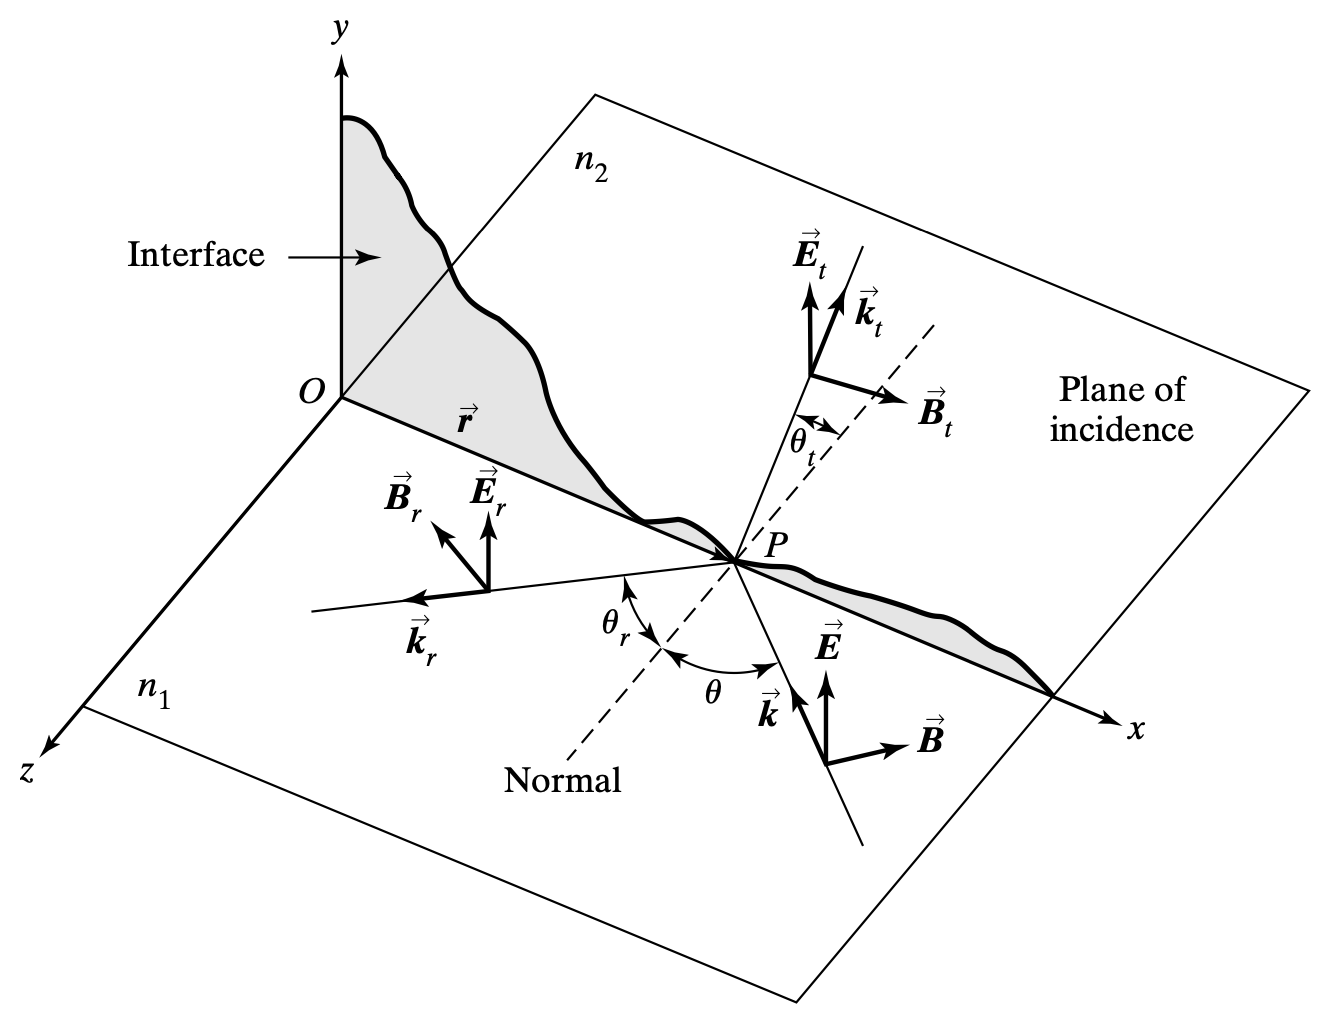
\includegraphics[width=0.8\textwidth]{Chapters/Figures/Incident, Relfected, and Transmitted Ray for TE Mode.png}
  \caption{The transverse electric (TE) set-up}
\end{figure}

Let us consider that the incident light comprises of plane harmonic waves:
\begin{equation} \label{Plane harmonic wave equation - incident}
\vec{\mathbf{E}} = \vec{\mathbf{E}_0} e^{i(\vec{\mathbf{k}} \cdot \vec{\mathbf{r}} - \omega t)}
\end{equation}
In our analytical approach, we will specifically examine a linearly polarized light wave, where the electric field vector $\vec{\mathbf{E}}$ is oriented perpendicular to the plane of incidence. According to the right-hand rule, this configuration places the magnetic field vector $\vec{\mathbf{B}}$ within the plane of incidence. This particular polarization is known as the \textit{transverse electric} (TE) mode

The reflected and transmitted waves can then also be expressed as plane harmonic wave equations:
\begin{equation} \label{Plane harmonic wave equation - reflected}
\vec{\mathbf{E}_r} = \vec{\mathbf{E}_{0r}} e^{i(\vec{\mathbf{k_r}} \cdot \vec{\mathbf{r}} - \omega_r t)}
\end{equation}

\begin{equation} \label{Plane harmonic wave equation - refracted}
\vec{\mathbf{E}_t} = \vec{\mathbf{E}_{0t}} e^{i(\vec{\mathbf{k_t}} \cdot \vec{\mathbf{r}} - \omega_t t)}
\end{equation}

At the interface where all three waves emerge simultaneously, a crucial boundary condition must be established to govern the relationship between their respective wave amplitudes. This boundary condition stipulates that the waves both incident upon and emerging from the plane of incidence should exhibit continuity and differentiability. This requirement is contingent upon the assumption that the interface is isotropic.

\subsection{Boundary Conditions for TE Waves}
In the context of our TM mode configuration, we can express the wave equations for the incident, reflected, and transmitted electric field components waves as follows:
\begin{align*}
\vec{\mathbf{E}_0} &= E\hat{y}           &  \vec{\mathbf{E}_{0r}} &= E_r\hat{y}               &  \vec{\mathbf{E}_{0t}} &= E_t\hat{y}
\end{align*}
where $E$, $E_r$, and $E_t$ denote the complex field amplitudes corresponding to the incident, reflected, and transmitted waves, respectively. These wave equations adhere to the boundary conditions, ensuring the continuity of electric field components parallel to the interface, as in:
\begin{equation} \label{Electric field boundary conditions for TE waves}
E + E_r = E_t
\end{equation}

By basic trigonometry and Maxwell's equations, we can find the corresponding magnetic fields to be:
\begin{align*} 
\vec{\mathbf{B}} &= (B\mathrm{cos}(\theta \hat{x}) - B\mathrm{sin}(\theta \hat{z})) e^{i(\vec{\mathbf{k}} \cdot \vec{\mathbf{r}} - \omega t)} \\
\vec{\mathbf{B}}_r &= (-B_r\mathrm{cos}(\theta_r \hat{x}) - B_r\mathrm{sin}(\theta_r \hat{z})) e^{i(\vec{\mathbf{k_r}} \cdot \vec{\mathbf{r}} - \omega t)} \\ 
\vec{\mathbf{B}}_t &= (B_t\mathrm{cos}(\theta_t \hat{x}) - B_t\mathrm{sin}(\theta_t \hat{z})) e^{i(\vec{\mathbf{k_t}} \cdot \vec{\mathbf{r}} - \omega t)}
\end{align*}

As the magnetic field vector lies transversely to the plane of incidence, adherence to the boundary conditions necessitates the connection of parallel components of the magnetic field, as defined by:
\begin{equation} \label{Magnetic field boundary conditions for TE waves}
B\mathrm{cos}(\theta) - B_r\mathrm{cos}(\theta) = B_t\mathrm{cos}(\theta_t) 
\end{equation}
Here, it's important to note that $\theta = \theta_r$ according to the law of reflection. Equations \ref{Electric field boundary conditions for TE waves} and \ref{Magnetic field boundary conditions for TE waves} stand as two pivotal equations arising from the boundary conditions for TE waves. These equations, instrumental in determining $R$, serve as a critical foundation. Nevertheless, before we delve into the calculation of $R$ through these boundary conditions, it is imperative to demonstrate the applicability of the same procedure to the transverse magnetic case.

\subsection{Boundary Conditions for TM Waves}
Another polarization mode for electromagnetic waves is known as the \textit{transverse magnetic} (TM) polarization. In this mode, the magnetic field vector is oriented perpendicular to the plane of incidence, while the electric field vector lies transverse to the plane of incidence. Within the framework of our TM mode configuration, we can formulate the wave equations governing the electric field components of the incident, reflected, and transmitted waves as follows:
\begin{align*} 
\vec{\mathbf{E}} &= (E\mathrm{cos}(\theta \hat{x}) - E\mathrm{sin}(\theta \hat{z})) e^{i(\vec{\mathbf{k}} \cdot \vec{\mathbf{r}} - \omega t)} \\
\vec{\mathbf{E}}_r &= (E_r\mathrm{cos}(\theta_r \hat{x}) + E_r\mathrm{sin}(\theta_r \hat{z})) e^{i(\vec{\mathbf{k_r}} \cdot \vec{\mathbf{r}} - \omega t)} \\ 
\vec{\mathbf{E}}_t &= (E_t\mathrm{cos}(\theta_t \hat{x}) - E_t\mathrm{sin}(\theta_t \hat{z})) e^{i(\vec{\mathbf{k_t}} \cdot \vec{\mathbf{r}} - \omega t)}
\end{align*}
Consequently, the magnetic field components can be written as:
\begin{align*}
    \vec{\mathbf{B}} &= -B\hat{y} e^{i(\vec{\mathbf{k}} \cdot \vec{\mathbf{r}} - \omega t)} \\
    \vec{\mathbf{B}}_r &= B_r\hat{y} e^{i(\vec{\mathbf{k}} \cdot \vec{\mathbf{r}} - \omega t)} \\
    \vec{\mathbf{B}}_t &= -B_t\hat{y} e^{i(\vec{\mathbf{k_t}} \cdot \vec{\mathbf{r}} - \omega t)} \\
\end{align*}

% inserting the TM wave example
\begin{figure}
  \centering
  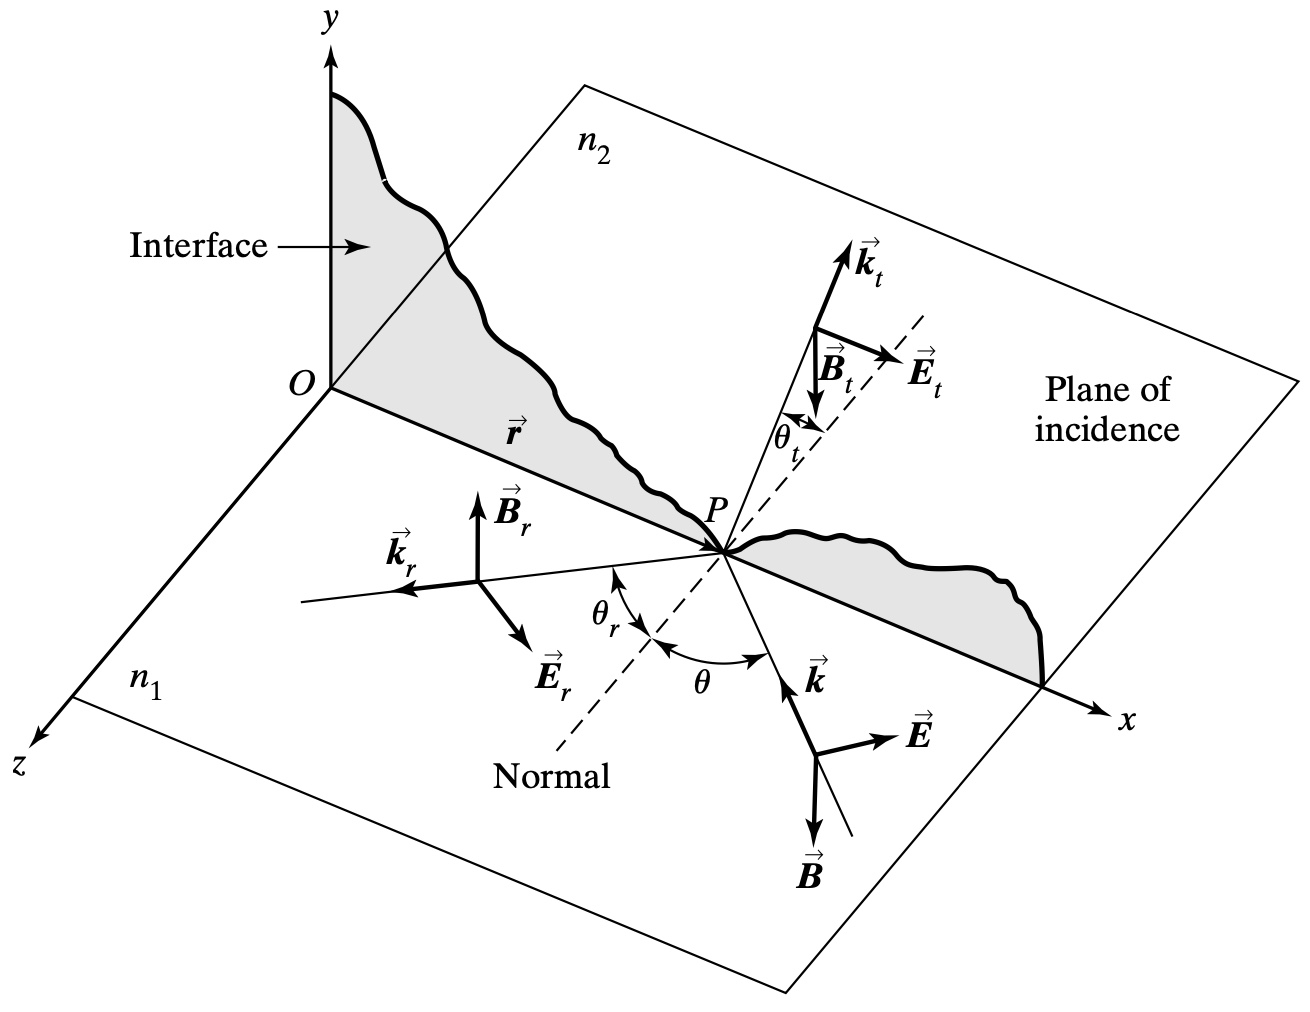
\includegraphics[width=0.8\textwidth]{Chapters/Figures/Incident, Relfected, and Transmitted Ray for TM Mode.jpg}
  \caption{The transverse electric (TM) set-up}
\end{figure}

These equations adhere to the boundary conditions, guaranteeing the continuity of electric field components parallel to the interface, as demonstrated by:
\begin{equation} \label{Magnetic field boundary conditions for TM waves}
-B + B_r = -B_t
\end{equation}

\begin{equation} \label{Electric field boundary conditions for TM waves}
Ecos(\theta) + E_rcos(\theta) = E_tcos(\theta_t)
\end{equation}

% REFLECTION AND TRANSMISSION COEFFICIENTS
\subsection{Reflection and Transmission Coefficients}
To determine the reflectance $R$ and, consequently, the transmittance $T$, it is imperative to define the reflection and transmission coefficients, as follows:
\begin{equation} \label{Definition of the reflection coefficient}
r = \frac{E_r}{E}
\end{equation}
and
\begin{equation} \label{Definition of the transmission coefficient}
t = \frac{E_t}{E}
\end{equation}

However, it is essential to calculate these coefficients for both the TE and TM cases. Recall that the electric and magnetic field amplitudes are linked through the following relation:
\begin{equation} \label{Equation relating the electric and magnetic field amplitudes}
E = \nu B = (\frac{c}{n})B
\end{equation}

We can employ \ref{Equation relating the electric and magnetic field amplitudes} to replace every occurrence of \(B\) in the boundary conditions with its corresponding \(E\). Initiating with the TE case, remember the two vital boundary condition equations for the TE mode:
\begin{equation}
TE:
\begin{cases} \label{TE boundary conditions}
  E + E_r = E_t \\
  n_1Ecos(\theta) - n_1E_rcos(\theta) = n_2E_tcos(\theta_t)
\end{cases}
\end{equation}
We can proceed to solve the system of equations above for the TE case to determine $r_{TE}$ (by eliminating all instances of $E_t$). Introducing the concept of the \textit{relative refractive index}, denoted as $n$ and defined as $n \equiv \frac{n_2}{n_1}$, we can derive:

\begin{equation} \label{Reflection coefficient (TE) in terms of n}
r_{TE} = \frac{E_r}{E} = \frac{cos(\theta) - ncos(\theta_t)}{cos(\theta) + ncos(\theta_t)}
\end{equation}
By the law of refraction, $sin(\theta) = nsin(\theta_t)$, we can eliminate $\theta_t$ by noting that:
\begin{equation} \label{Replacing \theta_t using the law of refraction}
ncos(\theta_t) = n \sqrt{cos^{2}(\theta_t)} = n\sqrt{1 - sin^2(\theta_t)} = \sqrt{n^2 - sin^2(\theta)}
\end{equation}
Finally, our $r_{TE}$ is:
\begin{equation} \label{Reflection coefficient (TE) without \theta_t}
r_{TE} = \frac{E_r}{E} = \frac{cos(\theta) - \sqrt{n^2 - sin^2(\theta)}}{cos(\theta) + \sqrt{n^2 - sin^2(\theta)}}
\end{equation}

Likewise, employing our boundary conditions for the TM case along with \ref{Equation relating the electric and magnetic field amplitudes}, we arrive at the reevaluated boundary conditions for the TM mode, which are as follows:
\begin{equation}
TM:
\begin{cases} \label{TM boundary conditions}
  -n_1E + n_1E_r = -n_2E_t \\
  Ecos(\theta) + E_rcos(\theta) = E_tcos(\theta_t)
\end{cases}
\end{equation}
With this revised form of the boundary condition, we can compute $r_{TM}$ in a manner similar to our determination of $r_{TE}$, resulting in:
\begin{equation} \label{Reflection coefficient (TM) without \theta_t}
r_{TE} = \frac{E_r}{E} = \frac{-n^2cos(\theta) + \sqrt{n^2 - sin^2(\theta)}}{n^2cos(\theta) + \sqrt{n^2 - sin^2(\theta)}}
\end{equation}
Similarly, if we follow the same steps we did for evaluating $r_{TM}$ and $r_{TE}$, we can subsequently figure out $t_{TM}$ and $t_{TE}$ (we now eliminate $E_r$ instead of $E_t$ ). We find:
\begin{equation} \label{Reflection coefficient (TM) without \theta_t}
t_{TE} = \frac{E_t}{E} = \frac{2cos(\theta)}{cos(\theta) + \sqrt{n^2 - sin^2(\theta)}}
\end{equation}

\begin{equation} \label{Reflection coefficient (TM) without \theta_t}
t_{TM} = \frac{E_t}{E} = \frac{2ncos(\theta)}{n^2cos(\theta) + \sqrt{n^2 - sin^2(\theta)}}
\end{equation}

Observing, for instance, the interconnection between $t_{TE}$ and $r_{TE}$, it is evident that they share the same denominator, suggesting that one can be expressed in terms of the other. To establish the relationship between the two equations, one can subtract $r_{TE}$ from $t_{TE}$, yielding 1. With some additional manipulation, the corresponding equation linking $t_{TM}$ and $r_{TM}$ can be derived. Ultimately, $r$ can be expressed in terms of $t$ as follows:
\begin{align*}
    t_{TE} &= 1 + r_{TE} \\
    nt_{TM} &= 1 - r_{TM} \\
\end{align*}
The set of equations $r_{TE}$, $r_{TM}$, $t_{TE}$, and $t_{TM}$ constitutes the \textbf{Fresnel Equations}. These equations provide reflection and transmission coefficients that establish the connection between incident and reflected energy field amplitudes in any linear, isotropic, and homogeneous medium. The primary objective of the Fresnel equations is to facilitate the determination of Reflectance $R$ and Transmittance $T$, which will be discussed in the subsequent subsection.

\subsection{Reflectance and Transmittance}
For energy conservation purposes, at a given boundary, the power incident on the boundary must be equal to the reflected and transmitted power at that boundary.
\begin{equation} \label{power balance equation at boundary}
P_i = P_r + P_t
\end{equation}

Finally, if we define reflectance $R$ and transmittance $T$ as:
\begin{equation} \label{Reflectance}
R = \frac{P_r}{P_i}
\end{equation}
\begin{equation} \label{Transmittance}
T = \frac{P_t}{P_i}
\end{equation}
So, $R$ is the ratio of the reflected to incident power while transmittance $T$ is the ratio of the transmitted to incident power. This means that \ref{power balance equation at boundary} takes the form of the famous unity equation (assuming no absorption):
\begin{equation} \label{R+T=1}
R + T = 1
\end{equation}
Power can be defined as the irradiance of the electromagnetic wave multiplied by the cross-sectional area traversed by the same wave. As in:
\begin{equation} \label{power balance equation in terms of irradiance}
I_iA_i = I_rA_r + I_tA_t
\end{equation}
To determine $A_i$, $A_r$, and $A_t$, we need to determine the cross-sectional area spanned by the incident, reflected, and transmitted electromagnetic waves respectively.

% Including the CSA example for the incident, reflected, and transmitted electromagnetic waves
\begin{figure}
  \centering
  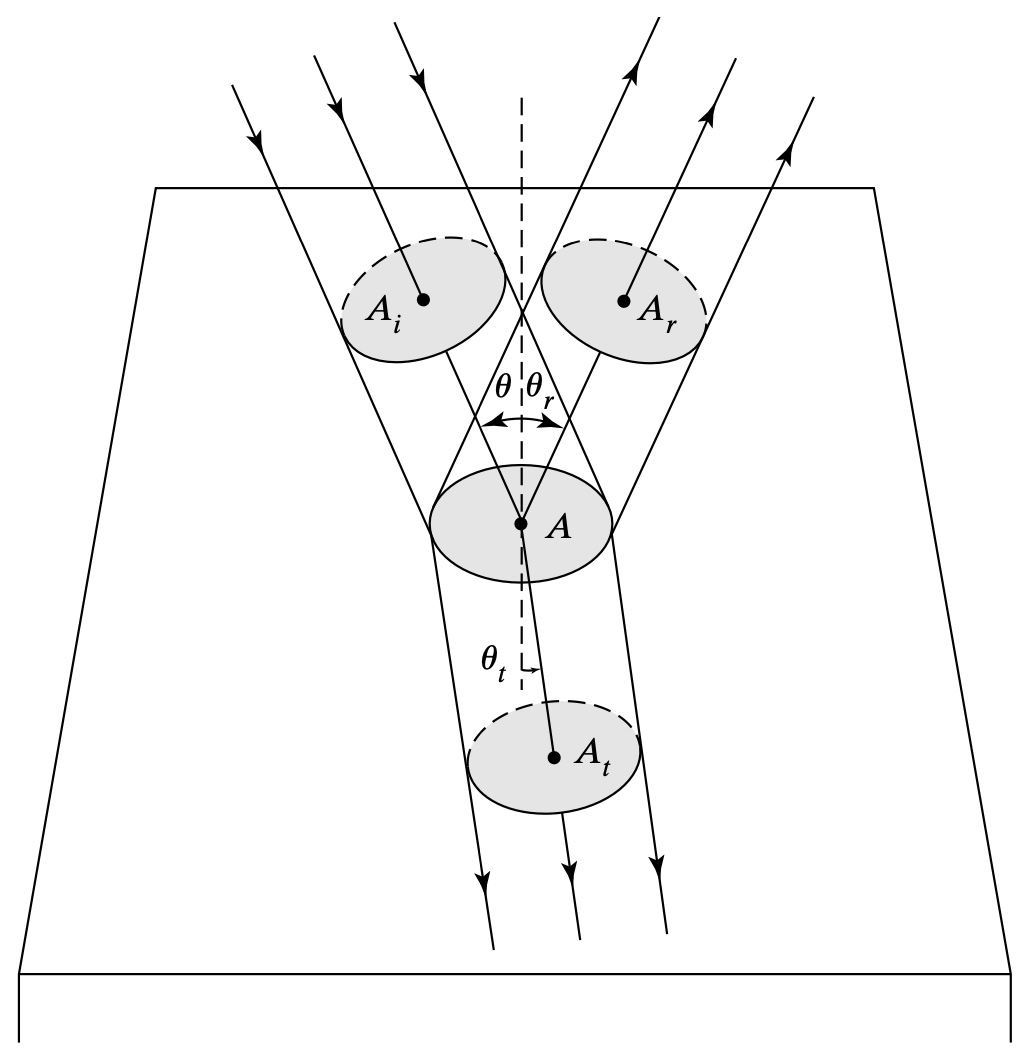
\includegraphics[width=0.8\textwidth]{Chapters/Figures/CSA Example for the Incident, Reflected, and Transmitted Electromagnetic Waves.jpg}
  \caption{The transverse electric (TM) set-up}
\end{figure}
